\subsection{Linear Models}
\label{sec:linear_models}

This section comprises results of linear engagement prediction models that
were trained as a baseline for later comparison with deep neural networks.
This kind of model evolution allows analysis of performance improvements
with regard to standardized metrics.
As is the case for all models, both multi-class classification and regression
models were developed for all data sets.
This section starts with describing the model architecture (ch.~\ref{sub:lin_architecture}) and continues by detailling the training process (ch.~\ref{sub:lin_training}).
It concludes by summarizing results and analyzing model performance in more detail
(ch.~\ref{sub:lin_performance}).

\subsubsection{Model architecture}
\label{sub:lin_architecture}

\begin{figure}[h]
  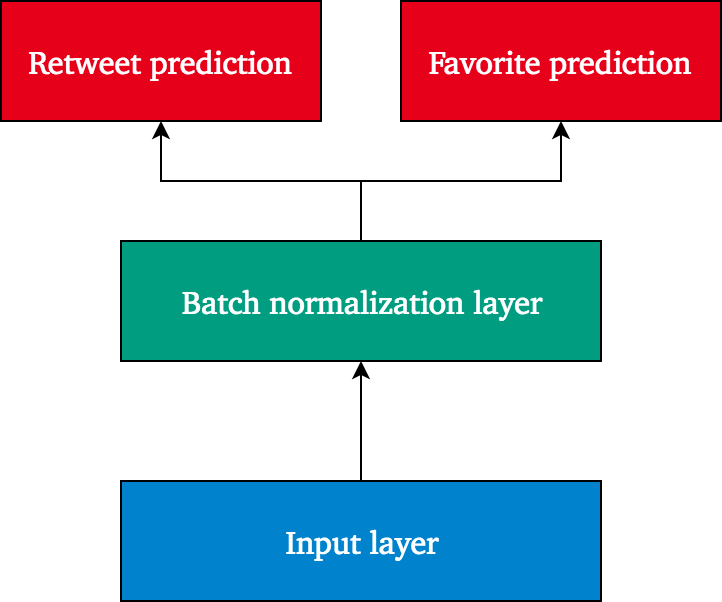
\includegraphics[height=8cm]{img/linear_model_architecture}
  \caption{General architecture of linear models}
\label{fig:linear_model_architecture}
\end{figure}

Fig.~\ref{fig:linear_model_architecture} illustrates the general architecture
of linear models trained in this work.
Firstly, inputs are normalized using a \textit{batch normalization} (see ch.~\ref{sub:dl_regularization})
layer in order to account for different scaling in the features.
As stated before, this layer type allows the model to undo normalization at
training time if it serves the purpose of better output representation.
The normalized inputs are then directly mapped onto two distinct outputs,
one for the number of retweets and one for the number of favorites.
In this case, regression and classification models only differ in their
respective type of prediction.
The regression model simply outputs two numbers representing retweet and
favorite estimates.
Hence, this constitutes a \textit{linear regression model}, because the output is not transformed.
Contrary, the classification model should output class probabilities for each
of the six predefined classes (see Table~\ref{tab:classification_buckets}).
As a result, the outputs have to be split according to the number of classes and transformed
using the \textit{sigmoid function} (see ch.~\ref{sub:dl_forward}).
This kind of model is called \textit{logistic regression} and considered
a linear classifier despite the outputs being transformed using a non-linear
function.
The reason for that is the sole reliance on a linear combination of the
(normalized) inputs.

\begin{table}
\begin{tabular}{ll}
\toprule
Feature & Description \\
\midrule
URL count & Number of URLs \\
Hashtag count & Number of hashtags \\
Mention count & Number of mentioned users \\
Tweet length & Length in characters \\
Quoted tweet & Is tweet a quote? \\
\midrule
Follower count & Number of followers the tweet author has \\
Friend count & Number of friends the tweet author has \\
Verified status & Is the tweet author verified? \\
User listings & Number of lists tweet author was added to \\
User tweet count & Total number of tweets by tweet author \\
User overall tweet frequency & Tweets per day by tweet author \\
User favorite count & Total number of given favorites by tweet author \\
User overall favorite frequency & Number of given favorites per day by tweet author \\
User account age & Number of days since account creation \\
Hour of tweet creation & Hour of the day the tweet was created \\
\bottomrule
\end{tabular}
\caption{Linear model features}
\label{tab:structured_features}
\end{table}

All input features (see Table~\ref{tab:structured_features}) are directly derived
from collected tweet objects.
Since these objects contain information about the tweet author, no further data lookups
are necessary.
Consequently, these features can be extracted with minimal preprocessing, which
enables model application in a real-time prediction setting.
The structured inputs are separated into content (top half) and contextual
features (bottom half).
Activity statistics, i.e. frequencies, are calculated on a per-day basis,
the hour of tweet creation is given in \textit{Coordinated Universal Time (UTC)}.
The previouly described need for normalization becomes obvious, e.g., when
comparing scales for URL counts (usually 0-3) and account age (thousands of days).
Content features mainly incorporate information on the use of conversational
tools (URLs, mentions, hashtags), but do not model the tweet content itself.
In addition, contextual features comprise popularity and activity information
about the tweet author.

\begin{table}
  \begin{tabular}{lr}
    \toprule
    Class & Range \\
    \midrule
    1 & 0 \\
    2 & 1-9 \\
    3 & 10-99 \\
    4 & 100-999 \\
    5 & 1,000-9,999 \\
    6 & >10,000 \\
    \bottomrule
  \end{tabular}
  \caption{Classes for classification models}
  \label{tab:classification_buckets}
\end{table}

General model output types were previously described.
In short, regression models output a positive real-valued estimate of the
eventual favorite and retweet count.
Classification models on the other hand aim to predict the probability that
these counts are within a certain range.
The prefined ranges represent the output classes and are shown in Table~\ref{tab:classification_buckets}.
Basically, the classes represent a logarithmic scale of eventual engagement counts.
Since retweet and favorite counts are wide-ranging in all three data sets,
scaling the outputs logarithmically creates a more balanced class distribution.
As described in section~\ref{sec:engagement_stats} the underlying class distributions
are still far from uniform.
However, the data sets proved to be large enough to learn this slightly 
imbalaced distribution with more complex models (see subsequent sections).
Other common methods for handling class imbalance, e.g., penalizing misclassifications
in rare classes via class weights, did not improve results significantly.
Retweet and favorite prediction are treated equally, i.e., the final loss
is calculated by building the mean of loss values for the singular tasks.

After establishing model architecture including input and output types, the next
session will explain details about the training process.

\subsubsection{Training process}
\label{sub:lin_training}

Accurate model comparisons require a standardized setting regarding training
processes.
Therefore, the following paragraphs will describe important aspects of model training
used in this work.
In particular, data usage, training duration and choices of optimization
algorithm and cost functions will be explained and motivated.

Prior to training, all three data sets were split into training and validation
data according to a 90\%/10\% split.
Since the splitting process was undertaken after permutating the example order
randomly, class distributions in training and validation sets should be very
similar.
Training examples were used to learn the weights of the model, whereas validation
examples are not known to the algorithm during training.
Consequently, the unseen data could be used to derive an estimate of the model
generalizability.
Models were trained for a fix number of iterations, each iteration consisting
of a full pass over all training examples.
Here, training data was split into batches of 128 examples whose gradients
were averaged in order to derive weight updates.
Testing was conducted to determine the required number of iterations for
convergence in loss function minimization.
The regression models turned out to converge slower, so that these models
had to be trained for a longer period of time.
In summary, regression models were trained for 150 iterations, whereas classification
models already converged after 50 iterations.

After comparing multiple optimization algorithms on data samples, \textit{adaptive
moment estimation (Adam)} was used for all experiments in this work.
Recapping from ch.~\ref{sub:dl_optimization_algos}, this recently developed
algorithm adapts learning rates for each parameter based on mean and variance of
recent updates.
It therefore combines strengths of previously developed techniques such as
\textit{momentum} and \textit{RMSprop}.
Tests showed faster convergence and more stability of the training process, i.e.,
fewer iterations were needed to derive an acceptable minimum of the loss function.
The default parameters detailed in the background chapter turned out to be sufficient
for linear models and did not require adjustments.

\textit{Adam} was applied to the minimization of two different cost functions for
classification and regression models.
Mathematical formulas and reasoning behind the choice of both functions
is outlined in the following.

\begin{equation}
  \label{eq:cross_entropy}
  C = -\frac{1}{n} \sum_x \sum_j y_j \ln a_j^L + (1 - y_j) \ln (1 - a_j^L)
\end{equation}

Evaluating performance of a classification model is mainly based on the ability
of the model to classify examples correctly.
Hence, the derived probability for the correct class should be close to one and
in that case, the value of the cost function for this example should be close
to zero (since cost functions are by definition minimized).
Equation~\ref{eq:cross_entropy} illustrates the \textit{categorical cross-entropy}
cost function. Here, $a_j^L$ represents the output of the last layer $L$ for class $j$,
evaluated on example $x$.
Intuitively, this is the probability estimate for example $x$ belonging to class $j$.
Cross-entropy calculates the natural logarithm of this estimate and multiplies
it with the desired output $y$, which is one if $x$ belongs to this class and
zero otherwise.
Thus, the cost for this example is derived from the first summand of the equation
if the example actually belongs to this class.
In the contrary case, the second summand determines the cost.
For both terms it holds, that the higher the difference between estimate and desired
output, the higher the value of the cost function will be (since the equation is negated).
The final cost for one example is derived by summing over all classes.
In order to calculate the loss value for one batch, the costs of all examples
in the batch are averaged.
Cross-entropy has come to be a standard cost function for classification
models, because it relies on probabilities and not just boolean values for class
membership.
Therefore, it allows more precise performance evaluation.
However, the metric is not interpretable directly.
Accordingly, results in this work will also list the metric \textit{accuracy}, which simply
denotes the percentage of correctly classified examples.
Results tables will abbreviate these metrics as \textit{CCE} and \textit{Acc}
respectively.

\begin{equation}
  \label{eq:mae}
  C = \frac{1}{n} \sum_x |y - a^L|
\end{equation}

A more directly interpretable cost function can be chosen for regression models.
Experiments in this work were conducted using \textit{Mean Absolute Error (MAE)},
which constitutes the average deviation between actual and desired outputs
in a batch of examples (see Equation~\ref{eq:mae}).
Interpretability was one of the reasons for choosing this metric over another popular alternative,
\textit{Root Mean Squared Error (RMSE)}.
Both metrics express an average prediction error in the respective variable unit,
here number of retweets or favorites.
However, MAE is more directly interpretable because output values
are not transformed at all and there is no distinction between error magnitudes.
By squaring error terms, RMSE penalizes large errors unproportionally higher
than small errors.
This is not desirable for the use case of this work, where underlying
engagement distributions come from a broad range of possible values.
\textit{Mean absolute percentage error (MAPE)} would have obvious benefits
on such a wide-ranging distribution, but it is not applicable in the existence
of zero values (which are present in all data sets).

\subsubsection{Model performance}
\label{sub:lin_performance}

After creating a standard setting for experiments across all data sets, 
results of training the linear models will be presented in this section.
Firstly, a summary of general performance metrics will be given, before
evaluating the classification models in more detail.
Finally, possible interpretations detected results will be listed.

\begin{table}
  \begin{tabular}{lrrrrrrr}
    \toprule
    & \multicolumn{4}{l}{Classification} & \multicolumn{3}{l}{Regression} \\
    \midrule
    Data set & CCE & Acc & Ret Acc & Fav Acc & MAE & Ret MAE & Fav MAE \\
    \midrule
    Celebrities & 1.22 & 48.84\% & 47.15\% & 50.52\% & 3,490.21 & 1,552.63 & 5,427.79 \\
    Politicians & 1.04 & 54.17\% & 51.64\% & 56.70\% & 482.81 & 273.83 & 691.80 \\
    Companies & 0.95 & 59.64\% & 63.38\% & 55.90\% & 24.66 & 13.02 & 36.29 \\
    Combined & 1.15 & 51.69\% & 54.00\% & 49.37\% & 579.26 & 269.35 & 889.16 \\
    \bottomrule
  \end{tabular}
  \caption{Summary of linear model results}
  \label{tab:lin_model_results}
\end{table}

Table~\ref{tab:lin_model_results} summarizes linear model results for all three
data sets.
For the classification task, both categorical cross-entropy (CCE) and
accuracy (Acc) metrics are given, regression performance is measured using
mean absolute error (MAE).
In addition, more detailed information about performance on the singular tasks of
retweet and favorite prediction is listed for the more interpretable metrics.
Data sets are staged in order of increasing data set size.
It can be generally observed that model performance improves with data set size, i.e.,
accuracy increases and loss values decrease.
For example, class predictions are 10\% more accurate for the company data set
than for celebrity tweets.
Moreover, retweet class predictions are more accurate than favorite class predictions
for celebrity and politician tweets.
Opposite behavior can be observed for the company data set.
For regression models, learning retweet prediction yields better results than
the counterpart task of predicting favorite counts.
However, this has to be expected since retweet counts are considerably smaller
and thus more narrowly distributed than favorites.
A wider underlying distribution of engagement counts, i.e., larger mean and median values, might also be the reason
for higher estimation discrepancies on celebrity and politician data.
Model performance on the larger, combined data set is comparable to the other
data sets.
This is hardly surprising, since the underlying class distribution constitutes a
weighted average of these examples.
For linear models, performance improvements from adding data can not be
expected due to the lack of representational capability.
In general, the observed results are not compelling for both classification and
regression models and leave room for improvements using deep neural networks.

\begin{figure}[h]
\begin{subfigure}{.5\textwidth}
  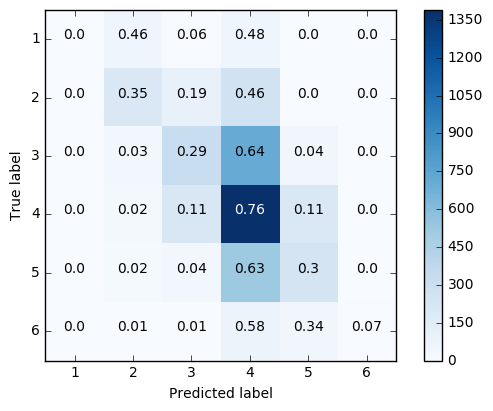
\includegraphics[width=.95\linewidth]{img/celeb_lin_cm_retweets}
  \caption{Celebrity data set}
  \label{fig:retw_distr_sub1}
\end{subfigure}%
\begin{subfigure}{.5\textwidth}
  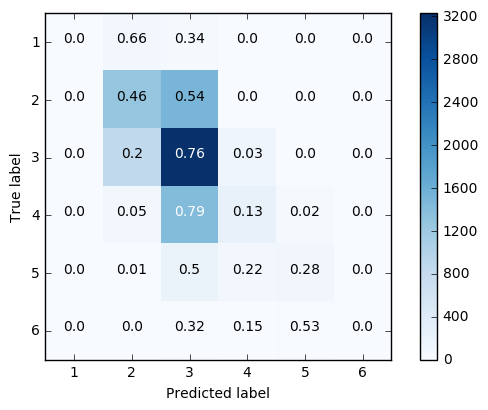
\includegraphics[width=.95\linewidth]{img/polit_lin_cm_retweets}
  \caption{Politician data set}
  \label{fig:retw_distr_sub2}
\end{subfigure}
\begin{subfigure}{.5\textwidth}
  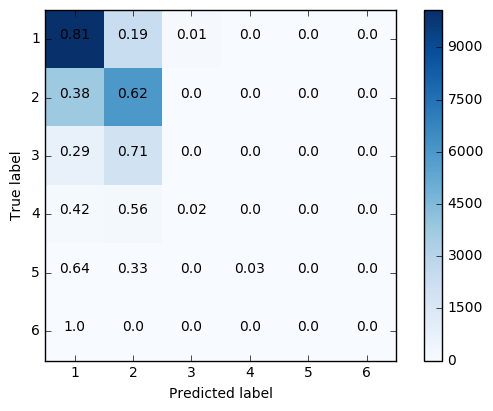
\includegraphics[width=.95\linewidth]{img/corp_lin_cm_retweets}
  \caption{Company data set}
  \label{fig:retw_distr_sub3}
\end{subfigure}%
\begin{subfigure}{.5\textwidth}
  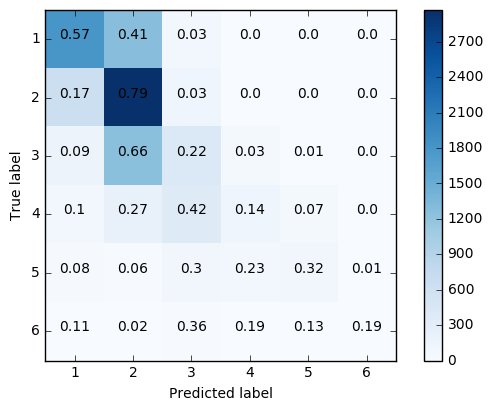
\includegraphics[width=.95\linewidth]{img/comb_lin_cm_retweets}
  \caption{Combined data set}
  \label{fig:retw_distr_sub3}
\end{subfigure}%
\caption{Confusion matrices for linear retweet classification models}
\label{fig:lin_cm}
\end{figure}

More detailed observations about classification performance can be derived from
looking at confusion matrices (see Fig.~\ref{fig:lin_cm}).
These illustrations contrast predicted and actual classes for all three data sets.
For example, entry $c_{ij}$ denotes which percentage of examples in class $i$
were placed in class $j$ by the classifier.
Hence, high percentages on the main diagonal are desirable for a solid classifier.
In addition to these normalized values, color maps illustrate the absolute
number of predictions for a particular class combination.
It can be stated that all models are biased towards larger classes, i.e.,
most examples are simply placed in these classes.
For celebrities, the most common class for celebrity tweets is 4 (100-999 retweets), while classes
3 (10-99 retweets) and 0 (zero retweets) are most frequently occurring for politician and company data
(see ch.~\ref{sec:engagement_stats}).
Accuracy for predicting these popular classes is higher than 75\% on all three data sets.
However, too many examples from other classes are misclassified here, as can be
seen when looking at respective class columns.
Such model behavior results in poor predictive performance for less common classes.
All observations also hold true for the combined data set, where classes 1 and 2
are predicted most accurately.
Confusion matrices for favorite prediction yield similar results and are
omitted for the sake of brevity here (see Appendix).

Analyzing above results points to an intuitive interpretation of model behavior.
All models are obviously biased towards the more common classes in a data set.
Since the company data possesses the most class imbalance (nearly 90\% of examples
stem from classes 0 and 1), linear models tend to perform better here.
Contrary, model performance decreases for wider and less imbalanced class distributions.
Two possible reasons for this kind of model bias can be derived.
Firstly, linear models have limited representational capability, i.e., a small
number of trainable parameters.
Secondly, structured input features could not be sufficient to learn acceptable
class boundaries.
For example, the actual tweet content is mostly ignored when using these simple
features.
The following sections will aim to overcome these liabilities by replacing
linear models with deep neural networks.
Adding more layers to the model architecture results in more trainable parameters
for representing inputs, which in turn should improve
model performance.
Results from training deep feedforward models on structured input data are
described in the following section (ch.~\ref{sec:deep1}).
Moreover, modeling tweet content using more sophisticated layer architectures
should enable deep neural networks to learn more meaningful features.
These additional features derived from unstructured data should also enable
more accurate engagement predictions.
Ch.~\ref{sec:deep_combined} explores possibilities for building these kinds
of more complex models.
